\documentclass[12pt]{article}
\newcommand{\bottomMargin}{2cm}


\newcommand{\header}{
	ДИЗАЙН И АНАЛИЗ НА АЛГОРИТМИ - \\ ПРАКТИКУМ\\
	\vspace{0.1cm}
	Летен семестър, 2026 г., второ контролно\\
	\vspace{0.1cm}
}
\newcommand{\tl}{$0.6$ сек.}
\newcommand{\ml}{$256$ MB}

\input{structure.tex}

\begin{document}
	
	\section{Задача К6. Магистрали}
	
	\begin{wrapfigure}{r}{0.30\textwidth}
	\begin{adjustbox}{width=0.30\textwidth}
		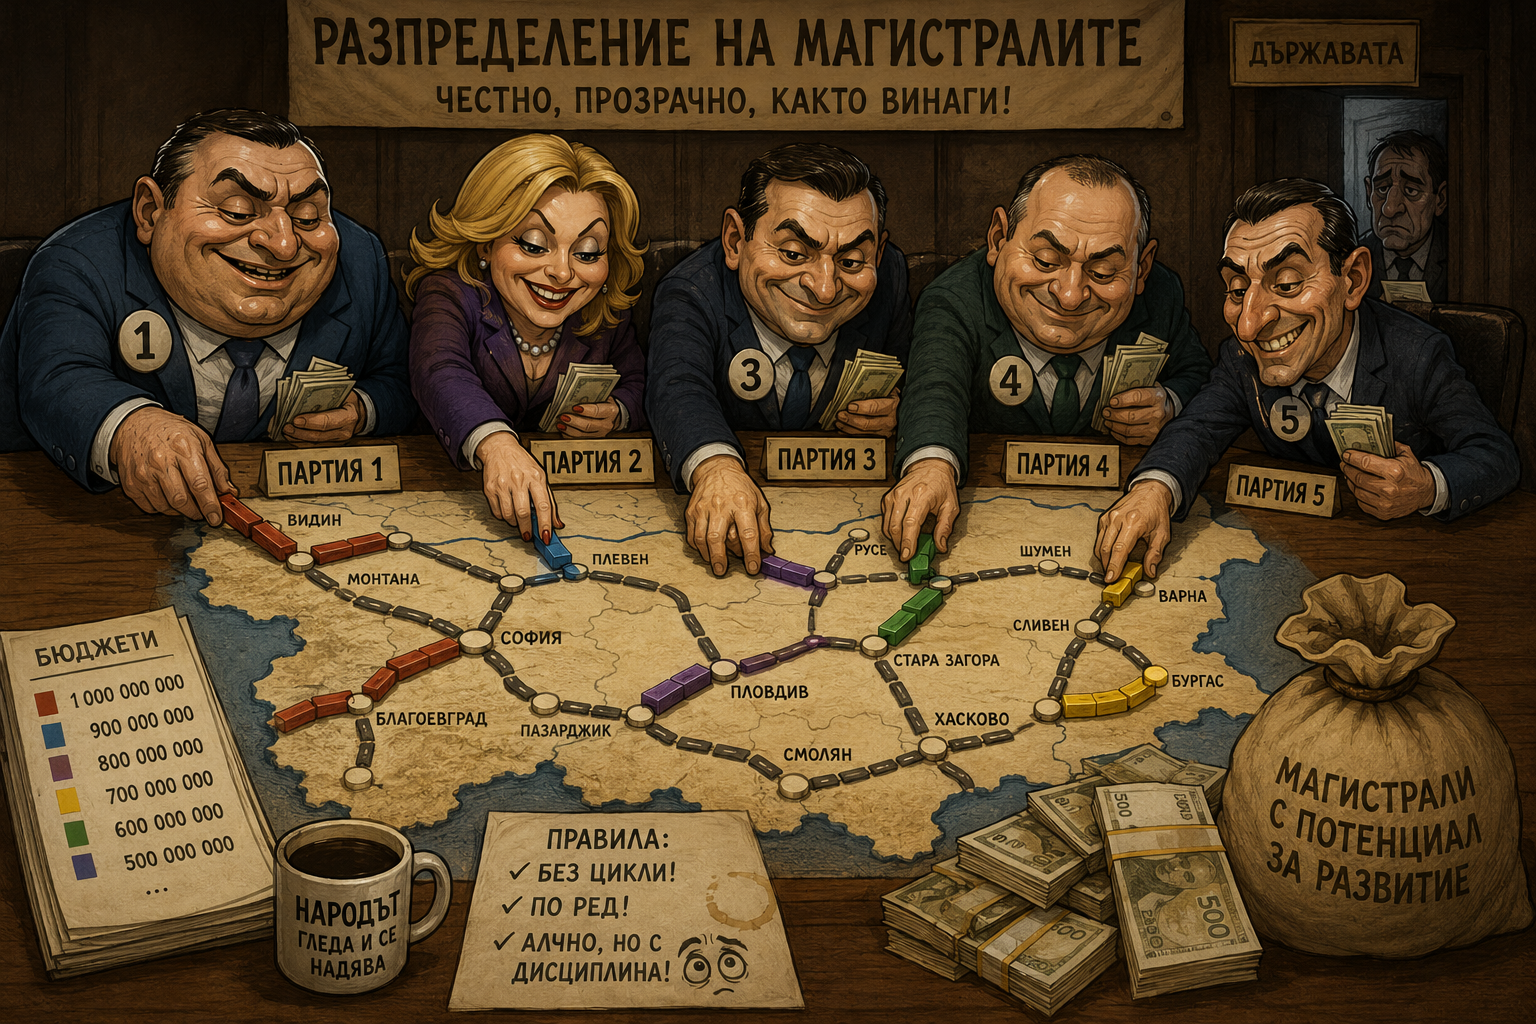
\includegraphics{image.png}
	\end{adjustbox}
    \end{wrapfigure}

	И ето, че след като резултатите от изборите са ясни е време за любимата на всички част -- разпределяне на корупционните схеми.
	
	В парламента влизат $K$ на брой партии, които искат да си разпределят парите за магистрали в България. В България има $N$ на брой града, номерирани с числата от $1$ до $N$. Планира се да се построят $M$ на брой магистрали, като $i$-тата от тях ще свързва двупосочно градовете $u_i$ и $v_i$, а парите, предвидени за нея са $w_i$. Тъй като различните отсечки са с различна сложност, бюджетите $w_1, \dots, w_M$ са \textbf{напълно различни} едни от други. Може да има повече от една магистрала, планирана между една и съща двойка градове.
	
	Сега партиите трябва да решат коя партия парите за кои магистрали ще открадне. Тъй като дори в най-порочните практики си има ред и дисциплина, партиите спазват стриктно следните правила:
	
	\begin{itemize}
		\item Партиите са номерирани от $1$ до $K$ спрямо тяхното влияние в парламента.
		\item Разпределението се случва последователно: първо партия $1$ избира набор от магистрали, които да присвои. След това партия $2$ избира от останалите неразпределени магистрали, и така нататък до партия $K$.
		\item Парите за дадена магистрала могат да бъдат откраднати от най-много една партия. Ако партия $j$ вече е взела дадена магистрала, никоя партия $k$ ($k > j$) не може да я вземе.
		\item За да не привличат вниманието на Европейската прокуратура с мащабни регионални монополи, никоя партия не може да открадне набор от магистрали, които образуват цикъл. Тоест, не трябва да е възможно да се тръгне от един град и да се стигне до същия, минавайки само по различни отсечки, откраднати от една и съща партия.
		\item Всяка партия е безкрайно алчна и избира своя набор от магистрали така, че общата сума на откраднатите от нея пари да бъде максимално голяма. Може да се докаже, че при тези условия изборът на всяка партия е уникален.
		\item Магистралите, които не бъдат откраднати от нито една партия, остават за държавата и се строят честно.
	\end{itemize}
	
	Напишете програма \texttt{\textbf{highways}}, която по дадени градове, бюджети за магистрали и брой партии, определя съдбата на всяка една магистрала.
	
	\subsection{Вход}
	На първия ред на стандартния вход са дадени три цели числа $N$, $M$ и $K$, разделени с интервал.\\
	На всеки от следващите $M$ реда са дадени по три цели числа $u_i$, $v_i$ и $w_i$, описващи поредната магистрала.
	
	\subsection{Изход}
	На стандартния изход отпечатайте $M$ реда. На $i$-тия ред изведете номера на партията, която ще открадне $i$-тата магистрала. Ако тя остава за държавата, изведете $0$.
	
	\subsection{Ограничения}
	\vspace{0.1em}
	\begin{itemize}
		\item $2 \leq N \leq 1000$
		\item $1 \leq M \leq 300\ 000$
		\item $1 \leq K \leq 10\ 000$ (виж секция оценяване)
		\item $1 \leq u_i, v_i \leq N$
		\item $u_i \neq v_i$
		\item $1 \leq w_i \leq 1\ 000\ 000\ 000$
		\item $w_i \neq w_j$ за всяко $i \neq j$
	\end{itemize}
	
	\subsection{Оценяване}
	\begin{itemize}
	    \item В тестове, носещи 32 точки, $K=1$.
	    \item В тестове, носещи общо 92 точки, $K \leq 10$.
	\end{itemize}
	
	\subsection{Примери}
	\begin{table}[ht]
		\begin{tblr}{|X[30,l]|X[20,l]|X[50,l]|}
			\hline
			\textbf{Вход} & \textbf{Изход} & \textbf{Обяснение на примера} \\
			\hline
			\texttt{3 5 2\\1 2 3\\1 2 1\\2 3 4\\2 3 6\\1 3 2} &
			\texttt{1\\0\\2\\1\\2} &
			{Партия $1$ избира измежду магистралите $\{1, 2, 3, 4, 5\}$. За да максимизира печалбата без да затваря цикъл, тя взима магистрали $1$ и $4$. Общата печалба е $3 + 6 = 9$. \newline
			\newline
			Партия $2$ избира измежду останалите $\{2, 3, 5\}$. Тя взима магистрали $3$ и $5$ за обща печалба $4 + 2 = 6$. \newline
			\newline
			Магистрала $2$ не е взета от никого и се предава на държавата.}\\
			\hline
			\texttt{3 6 5\\1 2 1\\1 2 2\\2 3 3\\2 3 4\\3 1 5\\3 1 6} &
			\texttt{4\\3\\2\\1\\2\\1} &
			{} \\
			\hline
		\end{tblr}
	\end{table}
	
\end{document}
